\documentclass[12pt]{report}
\usepackage[utf8]{inputenc}
\usepackage[english]{babel}
\usepackage{microtype}
\usepackage{libertine}
\usepackage{amsmath,amsthm}
\usepackage[varg]{newtxmath}
\usepackage{accents}
\usepackage[table,xcdraw]{xcolor}
\usepackage{setspace,graphicx,epstopdf}
\usepackage{marginnote,datetime,url,enumitem,subfigure,rotating}
\usepackage{todonotes}
\usepackage{xfrac}
\usepackage{multirow}
\usepackage{graphicx}
\usepackage[open,openlevel=1]{bookmark}
\usepackage[tikz]{bclogo}
\usepackage{enumitem}

\setlength{\parindent}{0ex}
\setlength{\parskip}{1em}%Espacement des par

\setlist[itemize]{topsep=-5pt}
\setlist[enumerate]{topsep=-5pt}

\newtheorem{theorem}{Theorem}[chapter]
\newtheorem{definition}{Definition}[chapter]
\newtheorem{remark}{Remark}[chapter]
\newtheorem{axiom}{Axiom}[chapter]
\newtheorem{lemma}{Lemma}[chapter]
\newtheorem{proposition}{Proposition}[chapter]

\setcounter{tocdepth}{1}


\newcommand{\ubar}[1]{\underaccent{\bar}{#1}}
\newcommand{\E}[1]{\operatorname{E}\left[#1\right]}
\newcommand{\V}[1]{\operatorname{Var}\left[#1\right]}
\newcommand{\cov}[1]{\operatorname{Cov}\left(#1\right)}
\newcommand{\Prob}[1]{\operatorname{Pr}\left[#1\right]}
\newcommand{\avg}[2]{\frac{#1}{#2} \sum_{i=#1}^{#2}}
\def\D{\mathrm{d}}
\newcommand{\know}{\operatorname{know}}

\newcommand{\smalltodo}[2][] {\todo[caption={#2}, size=\scriptsize,%
fancyline, #1]{\begin{spacing}{.5}#2\end{spacing}}}
\newcommand{\rhs}[2][]{\smalltodo[color=green!30,#1]{{\bf PS:} #2}}

\renewcommand\bcStyleTitre[1]{\textbf{#1}}

\begin{document}

\date{}
\title{\textbf{\huge{ECON7741 - Microeconomic Theory}}\\ \textit{Lecture Notes from Utku Ünver's lectures}}
\author{Paul Anthony Sarkis\\ Boston College} 
 
\maketitle

\tableofcontents

\chapter{Normal-Form Games with Perfect information}

\section{Nash Equilibrium}

A normal-form game is a strategic game in which each player chooses all his strategies once and for all, right when the game begins. Therefore, a normal-form game is a model of an event that occurs only once, where each players know everything about how the game can be played, where they are perfectly rational, and where they choose their actions simultaneously and independently. Another way to interpret this form is that there is no information set available to the players that could help anyone form expectations on the others' behaviour.

\begin{definition}[Normal-form game] A normal-form game is a triplet $G = (N, (S_i)_{i\in N}, (\succeq_i)_{i\in N})$ such that:\begin{itemize}
\item $N = \{1, 2, ..., n\}$ is a finite set of players. We'll use the index $i\in N$ to denote a player.
\item $S_i$ is a non-empty set of strategies for each player $i$. It contains all possible strategies that a player can choose from. The product set $S = \times_{i\in N} S_i$ is the strategy profile set. It contains all possible strategy profiles $s = (s_1, ..., s_n)$.
\item $\succeq_i$ is a preference relation defined on $S$.
\end{itemize}
\end{definition}

This definition summarizes what requirements are needed to analyze a game. We can add other elements in this definition to make describing games more clear.

First, we'll define the index $-i$ as the complement of $i$ or in words, the index designing all other players than $i$. For example, $s = (s_i, s_{-i})$ will be used to single out player $i$'s strategy and the others. In the same manner, $S_{-i} = \times_{j\neq i} S_j$ is the set of all strategy profiles for other players than $i$.

Second, as an alternative to the preference relation $\succeq_i$, we could define a payoff function $u_i(\cdot) : S\to \mathbb{R}$ that represents $\succeq_i$ on $S$ such that, for all $s, s'$ we have that $$s \succeq_i s' \Leftrightarrow u_i(s)\geq u_i(s')$$In that case we'll represent the normal-form game as $G = (N, (S_i)_{i\in N}, (u_i)_{i\in N})$.

Finally, in order to analyze the outcome of a game, we'll introduce the major concept of Game Theory as a whole: the Nash equilibrium.

\begin{definition}[Nash equilibrium]
A Nash equilibrium of a game $G$ is a strategy profile $s^* = (s_1^*, s_2^*, ..., s_n^*) \in S$ such that for all $i\in N$, $$(s_i^*, s_{-i}^*)\succeq_i (s_i, s_{-i}^*) \quad \forall s_i\in S_i $$Alternatively, we can define it in terms of the payoff function where $$ s_i^* = \operatorname{arg}\max_{s_i} u_i(s_i, s_{-i}^*) \quad \forall i\in N$$
\end{definition}

\subsection{Solving for a Nash equilibrium in pure strategies}

\begin{table}[ht!]
\centering
\begin{tabular}{cccc}
 &  & \multicolumn{2}{c}{\textbf{Prisoner 2}} \\ \cline{3-4} 
 & \multicolumn{1}{c|}{} & \multicolumn{1}{c|}{Don't confess} & \multicolumn{1}{c|}{Confess} \\ \cline{2-4} 
\multicolumn{1}{c|}{\multirow{2}{*}{\textbf{Prisoner 1}}} & \multicolumn{1}{c|}{Don't confess} & \multicolumn{1}{c|}{5 ; 5} & \multicolumn{1}{c|}{-10 ; 6} \\ \cline{2-4} 
\multicolumn{1}{c|}{} & \multicolumn{1}{c|}{Confess} & \multicolumn{1}{c|}{6 ; -10} & \multicolumn{1}{c|}{- 5 ; - 5} \\ \cline{2-4} 
\end{tabular}
\end{table}

\subsection{Best response correspondences}

\begin{definition}[Best response correspondence]
Let $G$ be a normal-form game. The best response correspondence $B_i : S_{-i} \twoheadrightarrow S_i$ of player $i$ is defined as: $$\forall s_{-i}\in S_{-i},\quad B_i(s_{-i}) = \{s_i \in S_i : (s_i, s_{-i}) \succeq_i (s_i',s_{-i}) \quad \forall s_i'\in S_i\} $$
\end{definition}
Hence, we can use this new concept to find an alternative definition to the Nash equilibrium.
\begin{definition}[Nash equilibrium in best response]
A Nash equilibrium of a game G is a strategy profile $s^* = (s_1^*, ..., s_n^*)$ such that, for all $i \in N$, $$s_i^*\in B_i(s_{-i}^*)$$
\end{definition}
In addition to the best response, we can define a more general correspondence defined on $S$ directly.
\begin{definition}[Augmented best response correspondence]
The augmented best response correspondence for player $i$ is $\beta_i : S\twoheadrightarrow S_i$ that we define as: $$\beta_i(s) = B_i(s_i)$$ Additionally, we define the best response vector correspondence $\beta : S\twoheadrightarrow S$ or alternatively $\beta = (\beta_i)_{i\in N}$ as: $$\beta(s) = \{s\in S :   s_i\in\beta_i(s)\quad \forall i\in N\}$$
\end{definition}

\begin{definition}[NE in augmented best response]
A Nash equilibrium of a game $G$ is a strategy profile $s^*$ such that $s^*$ is a fixed-point of the game augmented best response correspondence $\beta(\cdot)$. Formally, $s^*$ is a Nash equilibrium if $$s^*\in\beta(s^*)$$
\end{definition}

\section{Nash's existence theorem in pure strategies}

\subsection{Preliminaries}

\begin{definition}[Nonempty-valuedness]
A correspondence $\phi:S\twoheadrightarrow T$ is nonempty-valued if, for all $s\in S$, $\phi(s)\neq\varnothing$.
\end{definition}

\begin{definition}[Convex-valuedness]
A correspondence $\phi:S\twoheadrightarrow T$ is convex-valued if, for all $s\in S$, any $t,t'\in \phi(s)$ and all $\sigma\in(0,1)$, we have that $$t\sigma + t'(1-\sigma) \in \phi(s)$$
\end{definition}

\begin{definition}[Graph]
Let $\phi:S\twoheadrightarrow T$ be a correspondence. The graph of $\phi$ is the set $\Gamma^\phi \subseteq S\times T$ such that $$\Gamma^\phi = \{(s,t)\in S\times T : t\in\phi(s)\} $$
\end{definition}

\begin{definition}[Upper-hemicontinuity]
A correspondence $\phi:S\twoheadrightarrow T$ is upper-hemicontinuous if, \begin{itemize}
\item[(i)] Its graph $\Gamma^\phi$ is a closed set.
\item[(ii)] The image of any compact subset $A\subseteq S$, $\phi(A)$ is bounded.
\end{itemize} 
\end{definition}

\begin{definition}[Quasi-concavity]
A function $u_i:S\to \mathbb{R}$ is quasi-concave with respect to $s_i$ if for all $s_{-i}\in S_{-i}$, all $s_i, s_i'\in S_i$ and all $\sigma\in (0,1)$, we have: $$u_i(\sigma s_i + (1- \sigma)s_i, s_{-i})\geq \min\{u_i(s_i,s_{-i}),u_i(s_i',s_{-i})\}$$
\end{definition}

\begin{definition}[Convexity]
A set $T$ is convex if for all $t,t'\in T$ and all $\sigma\in (0,1)$, we have:$$t\sigma + t'(1 - \sigma)\in T$$ 
\end{definition}

\subsection{Kakutani's fixed-point theorem}

We use Kakutani's fixed point theorem to show that our best response correspondence vector indeed contains at least one fixed point, thus proving the existence of a Nash equilibrium in certain games.

\begin{theorem}[Kakutani's fixed point theorem]
Suppose $S$ is a non-empty, compact and convex subset of $\mathbb{R}^n$ and that $\beta:S\twoheadrightarrow S$ is a nonempty-valued, convex-valued and upper hemi-continuous correspondence. Then, there exists a fixed point $s^*\in S$ of $\beta$. Formally, $\exists s^*\in S : s^* \in \beta(s^*)$.
\end{theorem}

We can delve deeper into the meaning of each assumption required for the theorem and explain why they are indeed necessary and to what context they apply to games.\begin{itemize}
\item \textbf{Nonemptiness of $S$:} for obvious reasons, we need our strategy set to be non-empty. If it was, then we'd have no Nash equilibrium possible.
\item \textbf{Compactness of $S$:} we can show that open sets could contain no fixed point by an example. Suppose $S=[0,1)$, then $f(s) = \frac{s+1}{2}$ is a correspondence that contains no fixed point.
\item \textbf{Convexity of $S$:} again, we can show by example that this assumption is required. Imagine $S$ as being a disk with a hole at the center (i.e. the center is not in $S$). Then, $f$ being a rotation of less than 360 degrees would be a correspondence without fixed points.
\item \textbf{Nonempty-valuedness of $\beta$:} this assumption is also obviously required.
\item \textbf{Convex-valuedness of $\beta$:} by example, if $S = [0,1]$ define $\beta(s) = \{1\}$ for $s\in[0,0.5)$, $\beta(s) = \{0,1\}$ for $s = 0.5$ and $\beta(s) = \{0\}$ for $s\in (0.5,1]$. Then there is no fixed point for $\beta$.
\item \textbf{Upper-hemicontinuity of $\beta$:} if we slightly modify the example given just above so that $\beta(0.5) = 1$, then there is no fixed point of $\beta$.
\end{itemize}

\subsection{Nash's existence proof}

We can now prove that our definition of a game really satisfies all the assumptions and therefore that Kakutani's theorem applies.

First, we have to assume the for all player $i$, the strategy set $S_i$ is non-empty, compact and convex. Hence, $S = \times_{i\in N} S_i$ is also a non-empty, compact and convex set. Moreover, we'll assume that preferences $\succeq_i$ are continuous in $S$ and convex in $S_i$. These assumptions are particularly relevant to well-behaved games and rational agents.

Second, using Weierstrass's theorem, we can show that $\beta$ is a nonempty-valued correspondence.

\begin{theorem}[Weierstrass's maximum value theorem]
Let $Y\subset\mathbb{R}^n$ be non-empty and $X\subset\mathbb{R}^m$ be non-empty and compact. Suppose $u:X\times Y\to\mathbb{R}$ is a continuous function on $X$. Then, for each $y\in Y$, there exists a $x^*(y)\in X$ such that $u(x^*(y), y)\geq u(x,y)$ for all $x\in X$.
\end{theorem}

In our context, consider $X$ as $S_i$, $Y$ as $S_{-i}$ and $u_i(s_i, s_{-i})$. From Weierstrass's theorem, we can be sure that, for each $s_{-i}$ there exists an $s_i^*$ such that $u_i(s_i^*, s_{-i})\geq u_i(s_i, s_{-i}) \quad \forall s_i\in S_i$. Therefore, $B_i(s_{-i})$ contains at $s_i^*(s_{-i})$ and we conclude that $\beta(s)$ is non-empty.

Now turning to the upper-hemicontinuity of $\beta$, we use Bergé's theorem.

\begin{theorem}[Bergé's maximum theorem]
Let $Y\subset\mathbb{R}^n$ and $X\subset\mathbb{R}^m$ be non-empty and compact. Suppose $u:X\times Y\to\mathbb{R}$ is a continuous function. Consider the correspondence $\beta : Y\twoheadrightarrow X$ such that:$\beta(y) = \{x\in X:u(x,y)\geq u(x',y)\quad \forall x'\in X\}$. Then, $\beta$ is upper-hemicontinuous.
\end{theorem}

Letting $X = S_i$ and $Y = S_{-i}$, we can see that $\beta(s)$ is upper-hemicontinuous.

Finally, we show that $\beta$ is a convex-valued correspondence: fix an $s^*\in S$ and suppose that $s, s'\in\beta(s^*)$. Then, $$(s_i, s_{-i}^*)\sim_i(s_i',s_{-i}^*)\succeq_i (s_i'',s_{-i}^*) \text{ for all } s_i''\in S_i\text{ and for all }i\in N\text{.}$$We can use the convexity of $\succeq_i$ to show that for all $\sigma\in (0,1)$:$$(\sigma s_i + (1-\sigma)s_i',s_{-i}^*)\succeq_i (s_i, s_{-i}^*)\sim_i(s_i',s_{-i}^*)$$ Hence, $\sigma s_i + (1-\sigma)s_i'\in\beta_i(s^*)$. Similarly, we can show that $\sigma s + (1 - \sigma)s'\in \beta(s)$ for $s = (s_i)_{i\in N}$ and $s' = (s_i')_{i\in N}$.

We have proved Nash's existence theorem written below à la Debreu (1952):

\begin{theorem}[Debreu's existence theorem]
Suppose the game $G = (N, (S_i)_{i\in N}, (\succeq_i)_{i\in N})$ satisfies that:\begin{enumerate}
\item For all $i\in N$, $S_i$ is a non-empty, compact and convex subset of $\mathbb{R}^n$.
\item For all $i\in N$, $\succeq_i$ is a continuous preference relation in $S$ and convex in $S_i$.
\end{enumerate} Then, game $G$ has a Nash equilibrium in pure strategies.
\end{theorem}

\section{Nash equilibrium in mixed strategies}

\subsection{Mixed strategies}

% EXAMPLE PAPER-ROCK-SCISSORS

In the previous example, we have seen that a Nash equilibrium does not seem to exist. A way to extend the strategy set in order to find NE (in the Paper-Rock-Scissors in particular) is to allow for a probability distribution over the strategy set $S_i$. We refer to this as mixed strategies and to the game as a mixed extension.

\begin{definition}[Mixed strategy]
For each $i\in N$, a mixed strategy of $i$ is a function $\sigma_i : S_i \to [0,1]$ such that $\sum_{s_i\in S_i}\sigma_i(s_i) = 1$. The set of mixed strategies for player $i$ is denoted $\Delta S_i$ which is a $\vert S_i\vert - 1$ dimensions simplex. If for some $s_i\in S_i$, we have $\sigma_i(s_i) = 1$, the strategy $s_i$ is referred to as a pure strategy. The associated payoff function $u_i:\Delta S\to \mathbb{R}$ is defined as : $$\hat u_i(\sigma) = \sum_{s\in S}\left(\prod_{j\in N} \sigma_j(s_j)\right)u_i(s) $$
\end{definition}

\subsection{Nash's existence theorem in mixed strategies}

\begin{definition}[Nash equilibrium in mixed strategies]
A mixed strategy Nash equilibrium of a game $G$ is a Nash equilibrium of its mixed extension. Formally, it is a mixed strategy profile $\sigma^*\in \Delta S$ such that for all $i\in N$: $$\sigma_i(s_i) = \operatorname{arg}\max_{\sigma_i} \hat u_i(\sigma) $$
\end{definition}

\begin{theorem}[Nash, 1950]
Suppose that game $G = (N, (S_i)_{i\in N}, (u_i)_{i\in N})$ satisfies finiteness of strategy set $S_i$ for all $i\in N$. Then, $G$ has a Nash equilibrium in mixed strategies.
\end{theorem}

Before proving this theorem, let's discuss some interpretations of what that kind of equilibrium implies. First, in any NE $\sigma^*\in\Delta S$, for any $i$ and any $s_i$ such that $\sigma_i^*(s_i) > 0$, playing $s_i$ without mixing is a best response to $\sigma_{-i}^*$. That means that player $i$ is indifferent between any strategy that has a positive probability in the mixed NE: all strategies have the same payoff when the other players are mixing.

\subsection{Solving for a Nash equilibrium in mixed strategies}

% BoS in mixed strategies

% Cournot

\chapter{Solutions through Common Knowledge of Rationality}

\section{Knowledge operator and common knowledge}

\begin{definition}[Knowledge Operator]
Le $\mathcal{X}$ be a set of propositions and $\know(\cdot)$ be an operator on $\mathcal{X}$ such that $\know_i(\mathcal{X})$ is the set of propositions that player $i$ knows in $\mathcal{X}$. Let $X\in\mathcal{X}$ be a set of propositions in $\mathcal{X}$, $\know_i(\mathcal{X})$ is defined as follows: $$X\in\know_i(\mathcal{X})\text{ if:}$$\begin{itemize}
\item "$i$ knows $X$"$\in\mathcal{X}$
\item if $i$ knows $X$, then $X$ is true
\item if $i$ knows $X$, then $i$ knows that $i$ knows $X$
\item if $i$ does not know $X$, then $i$ knows that $i$ does not know $X$
\item if $i$ knows $X$, then $i$ knows all logical implications of $X$ (i.e. if $X\Rightarrow Y$ and $i$ knows $X$, then $i$ knows $Y$)
\end{itemize}
\end{definition}

This definition will allow us to set rules for games and allow agents to play according to the rules and to other players playing by the rules.

For example, we return to the typical Battle of Sexes game. Let $X = \{$BoS will be played according to the table below, each player will try to maximize their payoff $\}$.
\begin{table}[ht!]
\centering
\begin{tabular}{cccc}
 &  & \multicolumn{2}{c}{\textbf{M (Player 2)}} \\ \cline{3-4} 
 & \multicolumn{1}{c|}{} & \multicolumn{1}{c|}{Concert} & \multicolumn{1}{c|}{Soccer} \\ \cline{2-4} 
\multicolumn{1}{c|}{\multirow{2}{*}{\textbf{W (Player 1)}}} & \multicolumn{1}{c|}{Concert} & \multicolumn{1}{c|}{2 ; 1} & \multicolumn{1}{c|}{0 ; 0} \\ \cline{2-4} 
\multicolumn{1}{c|}{} & \multicolumn{1}{c|}{Soccer} & \multicolumn{1}{c|}{0 ; 0} & \multicolumn{1}{c|}{1 ; 2} \\ \cline{2-4} 
\end{tabular}
\end{table}

Following our definition of the knowledge operator, we can write:\begin{itemize}
\item If $W$ knows $X$, then $X$ is true and hence the game will be played by those rules with only rational players. 
\item If $W$ knows $X$, $W$ knows that $W$ knows $X$. \item If $W$ does not know $X$, then $W$ knows that $W$ does not know $X$. 
\item If $W$ knows  $X$, then $W$ knows all implications of $X$.
\end{itemize}

In order to solve the game, we'll need to assume that all players can play according to the rules and in a rational manner. This assumption will be defined by the concept of common knowledge.

\begin{definition}[Common knowledge]
$X\in\mathcal{X}$ is common knowledge among a set of agents $N$ if for all $i\in N$ and $j\in N\backslash\{i\}$:\begin{itemize}
\item $X\in\know_i(\mathcal{X})$: player $i$ knows $X$.
\item $(X\in\know_j(\mathcal{X}))\in\know_i(\mathcal{X})$: player $i$ knows that player $j$ knows $X$.
\item $((X\in\know_{j'}(\mathcal{X}))\in\know_{j}(\mathcal{X}))\in\know_i(\mathcal{X})$: player $i$ knows that player $j$ knows that any player $j'$ knows $X$.
\item $\hdots$, ad infinitum.
\end{itemize}
\end{definition}
\newpage

Back to the BoS game described above, the assumption of common knowledge would imply that: \begin{itemize}
\item $W$ knows $X$. $M$ knows $X$.
\item $W$ knows that $M$ knows $X$. $M$ knows that $W$ knows $X$.
\item $W$ knows that $M$ knows that both $W$ and $M$ know $X$. $M$ knows that $W$ knows that both $W$ and $M$ know $X$.
\item $\hdots$, ad infinitum.
\end{itemize}

This assumption of common knowledge, as well as the rationality of players are crucial to finding Nash equilibria in real situations. Of course there might be situations where common knowledge and/or rationality will fail, and we will see how to adress those issues later.

\section{Strategic Dominance}

In this section, we will study how common knowledge and rationality will help categorize strategies with regards to the likelihood that they'll be played. In particular, we will first define the concept of domination to represent strategies that are intrinsically better than others.

\begin{definition}[Strict domination]
Let $G$ be a strategic game. For any $i\in N$, a pure strategy $s_i\in S_i$ is \textbf{strictly dominated} if: $$\exists \sigma_i\in\Delta S_i \text{ such that } u_i(\sigma_i,s_{-i}) > u_i(s_i, s_{-i}) \text{ for all } s_{-i}\in S_{-i} $$ In this case, we say that $\sigma_i$ strictly dominates $s_i$.
\end{definition} 
In words, this definition means that for a given strategy $s_i$, if there exists at least one way to mix between strategies and get a strictly better payoff for all pure strategies played by the others, then $s_i$ is strictly dominated.

\begin{definition}[Weak domination]
Let $G$ be a strategic game. For any $i\in N$, a pure strategy $s_i\in S_i$ is \textbf{weakly dominated} if: $$\exists \sigma_i\in\Delta S_i \text{ such that } u_i(\sigma_i,s_{-i}) \geq u_i(s_i, s_{-i}) \text{ for all } s_{-i}\in S_{-i}$$ $$\text{ and } u_i(\sigma_i,s_{-i}) > u_i(s_i, s_{-i}) \text{ for some } s_{-i}$$ In this case, we say that $\sigma_i$ weakly dominates $s_i$.
\end{definition}
This definition is slightly weaker than the previous one since it allows for the dominated strategy to give the same payoff in some cases if there is at least one case where it is not the case.

\begin{definition}[Dominant strategy]
A strategy $s_i\in S_i$ is said to be strictly (weakly) dominant if it strictly (weakly) dominates all other strategies. By definition, a strictly dominant strategy must be a pure strategy.
\end{definition}

In the prisoner's dilemma game, the strategy to confess is a strictly dominant strategy for both prisoners since:\begin{itemize}
\item When prisoner $j$ confesses, prisoner $i$ is strictly better off by confessing as well ($-5 > -10$).
\item When prisoner $j$ does not confess, prisoner $i$ is strictly better off by confessing ($6 > 5$).
\end{itemize} This implies that under common knowledge and rationality, both players know that they have a dominant strategy to play and will play it. The Nash equilibrium is therefore at the crossing of strictly dominant strategies. Not all games contain strictly or weakly dominant or dominated strategies. For example, the game Rock-Paper-Scissors contains no such strategies.

We have seen a relationship between strict dominance and Nash equilibria in the prisoner's dilemma. What is the extent of this relationship? In order to answer this question, we'll have to define a few more elements.

\begin{definition}[Never-best-response strategy]
A strategy $s_i\in S_i$ is a never-best-response strategy if $s_i\not\in B_i(\Delta S_{-i})$.
\end{definition}

\begin{theorem}
Let $G$ be a game where $N=2$, then $s_i$ is strictly dominated if and only if it is a never-best-response strategy. 

For $N\geq 3$, a strictly dominated strategy is always a never-best-response while the converse is not true.
\end{theorem}

\section{Iterated elimination of dominated strategies}

\subsection{Definitions}

Since the previous section has shown us that some strategies are better than other, we can use this knowledge and look at how the game changes when we eliminate strategies that are dominated by others. Because there are three concepts of domination defined, we'll define three processes of strategy elimination.

\begin{definition}[Iterated elimination of strategies]
A set of strategy profiles $S^\infty\subseteq S$ survives iterated elimination of strictly dominated (weakly dominated) (never-best response) strategies if there exists a sequence of strategy profile sets $\{S^k\}_{k=1}^{\infty}\subseteq S$ such that, $G^{(1)} = G, S^{(1)} = S$ and for any $k>1$, $S^{(k)}$ is obtained by eliminating ALL strictly dominated (weakly dominated) (never-best response) strategies of all players in the game $G^{(k-1)} = \left(N, S_i^{(k-1)}, u_i^{(k-1)}\right)$; and $S^{(\infty)} = \bigcap_{k=1}^{\infty} S^{(k)}$. We'll denote this set by $S^{\text{IESDS}}$ ($S^{\text{IEWDS}}$) ($S^{\text{IENBRS}}$).
\end{definition} If this definition seems a bit too formal, translating it in words reveal the meaning is in fact pretty simple. Indeed, starting with $G^{(1)}$ being the initial game as well as $S^{(1)}$ the initial strategy set, we will advance to the next step by removing dominated strategies from $S^{(1)}$. The new strategy set is $S^{(2)}$ which gives the game $G^{(2)}$. We repeat this process by eliminating dominated strategies of $S^{(2)}$ to get $S^{(3)}$, and again from $S^{(3)}$ to get $S^{(4)}$ etc. The infinite set described in the definition is the limit of the process (i.e. what happens if we repeat the elimination an infinite number of times). 

\begin{definition}[Rationalizable strategy profiles]
The resulting set of Iterated Elimination of Strictly Dominated Strategies, $S^{\text{IESDS}}$, is known as the set of rationalizable strategy profiles.
\end{definition}

\subsection{Properties of iterated eliminations}

The processes of iterated elimination have interesting properties to examine. For example, in the IESDS, it does not matter if we delete strictly dominated strategies all at once or step-by-step as required. However, this step-by-step process is necessary in both IEWDS and IENBRS. Another interesting property of IESDS is that there is no importance to "forgetting" to eliminate a SDS during one step, as long as you do it by the end of the process. Again, in IEWDS each round of elimination MUST get rid of ALL WDS. 

The three types however have no close link to common knowledge of rationality, this means we cannot say that one iterated elimination process is the unique one used by rational agents. In fact, rational agents can play weakly dominated strategies. 

Additionally, we have that:\begin{itemize}
\item $S^{\text{IEWDS}}\subseteq S^{\text{IESDS}}$.
\item $S^{\text{IENBRS}}\subseteq S^{\text{IESDS}}$ and for $N=2$, we even have $S^{\text{IENBRS}}= S^{\text{IESDS}}$.
\end{itemize}

%Cournot

\subsection{IESDS and Nash equilibria}

Going back to the prisoners' dilemma or the previous Cournot example, we see that IESDS seems to have a strong link with Nash equilibria: let's try and explore that relationship.

Define $NE\subseteq \Delta S$ as the set of all Nash equilibria of a game. The set $S\cap NE$ is the set of all pure strategy Nash equilibria. Now define $\hat S_i\subseteq S_i$ as the set of pure strategies of player $i$ such that there exists $\sigma = (\sigma_1, \sigma_2, ..., \sigma_n) \in NE $ where $\sigma_i(s_i)>0$. In words, $\hat S_i$ is the set of all strategies that are at least a part of a mixed strategy Nash equilibrium. In parallel, define $\hat S = \times_{i\in N} \hat S_i $.

\begin{proposition}
For any game $G$, we have: $$\hat S \subseteq S^{\text{IESDS}} $$
\end{proposition}

\begin{proof}

\end{proof}

\begin{lemma}
For any game $G$, any Nash equilibrium of $G$ can be found by looking at strategies and mixed strategies in $S^{\text{IESDS}}$.

\begin{proposition}
By the proposition and lemma above, for any game $G$, if $\vert S^{\text{IESDS}}\vert = 1$, then $$ S^{\text{IESDS}} = S\cap NE $$
\end{proposition}
\end{lemma}

\chapter{Extensive-Form Games with Perfect information}

We have seen in the first chapter the definition of normal-form games, or games that are played simultaneously by all players. Then we have seen concepts of Nash equilibrium in this particular types of games as well as dominant strategies, rationality, etc. This chapter has the goal of using these concepts to apply them to extensive-form games (i.e. games that are played sequentially).

\section{Definitions and equilibrium}

\begin{definition}[Extensive-form game]
An extensive-form game with perfect information is a quadruplet $G = (N, H, P, (u_i)_{i\in N})$ such that:\begin{itemize}
\item $N = {1, ..., n}$ is the set of players
\item $H$ is a set of finite or infinite sequences of actions ($a^1a^2 ...$) called histories such that:\begin{itemize}
\item $\emptyset \in H$: the beginning of the game is a history.
\item If $ha\in H$, then $h\in H$: if an action $a$ following a history $h$ is in $H$, then $h$ is also in $H$.
\end{itemize}
We could additionally define the set $H^\infty\subseteq H$ as the set of infinite histories. The set $H^T = \{h \in H\backslash H^\infty : \not\exists a, ha\not\in H\}$, the set of terminal histories. Finally, for any $h\in H\backslash H^T$, $A(h) = \{a : ha\in H\}$ is the set of all possible actions to play after the history $h$.
\item $P: H\backslash H^T \to N$ is a player function which designates the player who moves after each non-terminal history.
\item For every $i\in N$, $u_i:H^T\to \mathbb{R}$ is the payoff function as we have already seen it.
\end{itemize}
\end{definition}

This definition allows us to describe two types of sequential games with the same tools: infinite-horizon games and finite-horizon games. An infinite-horizon game is a game where the set of infinite histories $H^\infty \neq \emptyset$. Meanwhile, a finite-horizon game has the property of $H^\infty = \emptyset$.

Let's try to understand the basic definition of extended-form games with two examples. The first example is the game represented by the following figure:\begin{center}
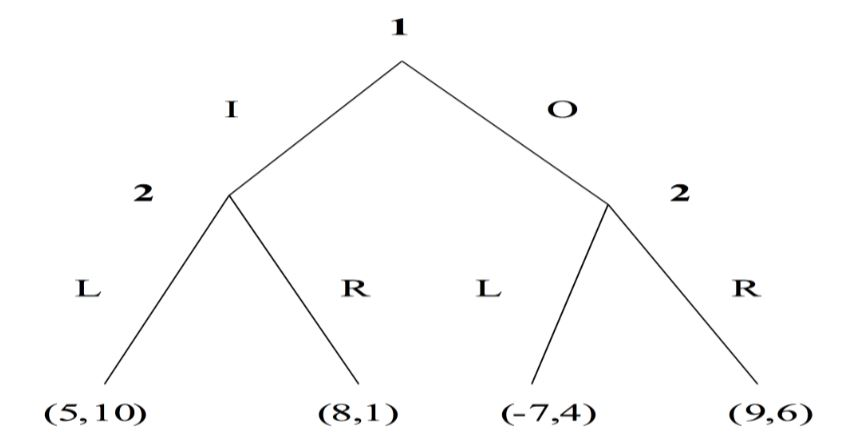
\includegraphics[scale=0.35]{images/LIORgame}
\end{center}
In this game, we have $N = 2$ for the two players that play. The set of all histories is $H = \{\emptyset, I, O, IL, IR, OL, OR\}$. There is no infinite history set. The set of all terminal histories is $H^T = \{IL, IR, OL, OR\}$. Hence we are left with the function: \begin{align*}
A(h) = \begin{cases}
\{I, O\} & \text{ if } h = \emptyset \\
\{L, R\} & \text{ if } h \in \{I,O\} 
\end{cases}
\end{align*}
The player function is defined in the same way: \begin{align*}
P(h) = \begin{cases}
1 & \text{ if } h = \emptyset \\
2 & \text{ if } h \in \{I,O\} 
\end{cases}
\end{align*}
Finally, the payoff functions $u_1$ and $u_2$ are described in the graph above.

For the second example, we focus on the Stackelberg model of competition, which can be represented by the following graph:

In this game, $N=2$, $H = \{\emptyset, [0, \infty), [0, \infty)[0, \infty)\}$. The set of terminal histories is $\mathbb{R}_+^2$. The function $A(h) = [0,\infty	)$ for all $h\in H\backslash H^T$ and the player function \begin{align*}
P(h) = \begin{cases}
1 & \text{ if } h = \emptyset \\
2 & \text{ if } h = [0, \infty) 
\end{cases}
\end{align*}
Finally, the payoff functions are defined by: $$u_i = (1 - q_i - q_{-i})q_i $$

These two games with only two steps are already interesting in how they are different from the games studied so far. Nevertheless, they share a lot in common as we can see by introducing the following concepts.

Let $H_i = \{h\in H\backslash H^T : P(h) = i\}$ be the set of histories at which it is player $i$'s turn to move. In parallel, let $A_i = \cup_{h\in H_i}A(h)$ define the set of all actions available to player $i$.

\begin{definition}[Strategy of an extended-form game]
For any $i\in N$, a strategy $s_i$ of the extended-form game $G$ is a function $s_i:H_i\to A_i$ such that for all $h\in H_i$, $s_i(h) \in A(h)$. We can define all concepts from the earlier chapters over that definition, such as $S_i$ the set of strategies for $i$, $S$ the set of all strategy profiles, etc.
\end{definition}

\begin{definition}[Outcome function]
Each strategy profile pins down a unique path in $G$ (a terminal history). Let $o:S\to H^T$ be this outcome function (i.e. $o(s)$ is the corresponding $H^T$ of playing $s$).
\end{definition}

\begin{definition}[Induced payoff function]
Let $u_i^*$ be the induced payoff function of player $i$, defined on $S$ such that for any $s,s'\in S$, $$ u_i^*(s)\geq u_i^*(s') \Leftrightarrow u_i(o(s))\geq u_i(o(s')) $$
\end{definition}

With these definitions in hand, we can represent the extended-form game as a normal-form game. And therefore define the Nash equilibrium of the extensive-form thanks to its normal-form representation.

\begin{definition}
For any extensive-form game with perfect information $G$, define $G^* = (N, (S_i)_{i\in N}, (u_i^*)_{i\in N})$ as the normal-form game induced by $G$.
\end{definition}

\begin{definition}[Nash equilibrium in a EFGPI]
A history $h^*\in H^T$ is a Nash equilibrium of an extended-form game with perfect information $G$ if and only if $s(h^*)$ is a Nash equilibrium of the normal-form game $G^*$ induced by $G$.
\end{definition}

Again, we will explain these new concepts with examples, starting with the first one of the chapter. 

First, the strategies of $G$ for both players are: $$A_1(\emptyset) = \{I, O\} \Rightarrow S_1 = \{I, O\} $$ $$A_2(I) = \{L, R\} ; A_2(O) = \{L, R\} \Rightarrow S_2 = \{L^IL^O, L^IR^O, R^IL^O, R^IR^O\} $$ $$\Rightarrow S = \{(I,L^IL^O), (I,L^IR^O), (I,R^IL^O), (I,R^IR^O), $$ $$ (O,L^IL^O), (O,R^IL^O), (O,L^IR^O), (O,R^IR^O)\} $$

The outcomes are: $$o((I,L^IL^O)) = o((I,L^IR^O)) = IL $$ $$o((I,R^IL^O)) = o((I,R^IR^O)) = IR $$ $$o((O,L^IL^O)) = o((O,R^IL^O)) = OL $$ $$o((O,L^IR^O)) = o((O,R^IR^O)) = OR $$

And hence we can present the payoffs in a normal-form game matrix: \begin{table}[ht!]
\centering
\begin{tabular}{cccccc}
 &  & \multicolumn{4}{c}{\textbf{Player 2}} \\ \cline{3-6} 
 & \multicolumn{1}{c|}{} & \multicolumn{1}{c|}{$L^IL^O$} & \multicolumn{1}{c|}{$L^IR^O$} & \multicolumn{1}{c|}{$R^IL^O$} & \multicolumn{1}{c|}{$R^IR^O$} \\ \cline{2-6} 
\multicolumn{1}{c|}{} & \multicolumn{1}{c|}{$I$} & \multicolumn{1}{c|}{\cellcolor[HTML]{C0C0C0}5 ; 10} & \multicolumn{1}{c|}{5 ; 10} & \multicolumn{1}{c|}{8 ; 1} & \multicolumn{1}{c|}{8 ; 1} \\ \cline{2-6} 
\multicolumn{1}{c|}{\multirow{-2}{*}{\textbf{Player 1}}} & \multicolumn{1}{c|}{$O$} & \multicolumn{1}{c|}{-7 ; 4} & \multicolumn{1}{c|}{\cellcolor[HTML]{C0C0C0}9 ; 6} & \multicolumn{1}{c|}{-7 ; 4} & \multicolumn{1}{c|}{\cellcolor[HTML]{C0C0C0}9 ; 6} \\ \cline{2-6} 
\end{tabular}
\end{table}

where greyed cells of the matrix are the Nash equilibria of $G^*$ and thus $G$.

\section{Subgame perfection}

\subsection{Definition and example}

In the last example, we have seen three Nash equilibria. However, from the design of the game it is clear that player 1 will never play $I$ in this situation since playing $O$ will always give him a higher payoff. We call the Nash equilibrium $(I, L^IL^O)$ not sequentially rational.

\begin{definition}[Subgame]
A subgame of an extensive-form game with perfect information $G = (N, H, P, (u_i)_{i\in N})$ at a non-terminal history $h\in H\backslash H^T$, is an extensive-form game with perfect information $G\vert_h = (N\vert_h, H\vert_h, P\vert_h, (u_i\vert_h)_{i\in N\vert_h})$ where:\begin{itemize}
\item $H\vert_h = \{h' : hh'\in H\}$: the set of histories starting from $h$.
\item $N\vert_h = \{i\in N : P(hh') = i\text{ for some } h'\in H\vert_h\backslash H^T\vert_h\}$: the set of players who have to play after $h$ has been realized.
\item $P\vert_h: H\vert_h\to N\vert_h$ such that for all $h'\in H\vert_h$, $P\vert_h(h') = P(hh')$.
\item For each $i\in N\vert_h$, $u_i\vert_h : H^T\vert_h\to\mathbb{R}$ such that for all $h'\in H^T\vert_h$, $$u_i\vert_h(h') = u_i(hh')$$
\end{itemize}
\end{definition}

\begin{definition}[Subgame-perfect Nash equilibrium]
A strategy profile $s = (s_1, ..., s_n)$ is a subgame-perfect Nash equilibrium (SPNE) of an extensive-form game with perfect information $G$ if for all $h\in H\backslash H^T$, $s\vert_h = (s_1\vert_h, ..., s_n\vert_h)$ is a Nash equilibrium of the subgame $G\vert_h$.
\end{definition}

Without any surprise, we will rely on the previous example to grasp a better understanding of the two new concepts. In that game there are three subgames:\begin{itemize}
\item $G\vert_\emptyset = G$: the game itself.
\item $G\vert_I = \left(\{2\}, \{\emptyset, L, R\}, [P(\emptyset) = 2], [u_2(L) = 10, u_2(R) = 1]\right)$: the game following the $I$ move from player 1.
\item $G\vert_O = \left(\{2\}, \{\emptyset, L, R\}, [P(\emptyset) = 2], [u_2(L) = 4, u_2(R) = 6]\right)$: the game following the $O$ move from player 1.
\end{itemize}

By backward induction we can solve for the SPNE:\begin{itemize}
\item In $G\vert_O$, player 2 will play $R$ since $u_2(L) = 4 < u_2(R) = 6$. $R$ is the NE of $G\vert_O$.
\item In $G\vert_I$, player 2 will play $L$ since $u_2(L) = 10 < u_2(R) = 1$. $L$ is the NE of $G\vert_I$.
\item In $G\vert_\emptyset$, player 1 will choose $O$ and go to subgame $G\vert_O$ because it yields a higher payoff that $G\vert_I$.
\end{itemize}

Only one SPNE exists: $(O, L^IR^O)$.

\subsection{Existence theorem}

As before, we are interested in proving the existence (under some conditions) of SPNEs in the context of extended-form games with perfect information. Also as previously done, we will give some preliminaries before the intuition.

For any positive integer $k$ smaller than the length of a given history $h$, let $h^k$ denote the history with the same first $k$ stages as $h$. If $k$ is bigger than the length of $h$, then $h^k$ is undefined.

\begin{definition}[Continuity of payoffs]
An infinite-horizon extensive-form game with perfect information $G = (N, H, P, (u_i)_{i\in N} )$ has the property of continuity of payoffs if for all $i\in N$: $$\lim_{k\to\infty} \sup_{h, h'\in H^T : h^k = h^{'k}} \vert u_i(h) - u_i(h')\vert = 0 $$ In words, continuity of payoffs means that as the number of common initial stages increase between two histories, the maximum difference in payoffs should tend to 0. 
\end{definition}

A typical situation in which this continuity of payoffs is satisfied is when players discount by a factor to the power of $k$. Then, for any $k>0$ and all $h^k\in H^T$, $u_i(h^k) = \delta^{k-1} v_i(h^k)$ where $\delta\in (0,1)$.

\begin{definition}[No profitable one-time deviation]
A strategy profile $s^*$ has the no profitable one-time deviation property if for every $i\in N$, and every $h\in H_i$ we have: $$u_i\vert_h (s_i^*\vert_h, s_{-i}^*\vert_h) \geq u_i\vert_h (s_i'\vert_h, s_{-i}^*\vert_h) $$ for all $s_i'\vert_h \in S_i\vert_h$ where $s_i'\vert_h(h') = s_i^*\vert_h(h')$ for all $h'\in H\vert_h$. This means that $s^*$ has this property if all strategy profiles where actions differ at one single point are weakly dominated by $s^*$ for all players.
\end{definition}

\begin{lemma}
Let $G$ be an extensive-form game with perfect information. Further assume that $G$ is either a finite-horizon game or an infinite-horizon game with continuity of payoffs. Then, the strategy profile $s^*$ is a SPNE of $G$ if and only if $s^*$ satisfies the no profitable one-time deviation property.
\end{lemma}

With these new concepts in mind, we can tackle the proof of existence to Kuhn's theorem.

\begin{theorem}[Kuhn's theorem of existence]
Every finite-horizon or infinite-horizon with continuity of payoffs extended-form game with perfect information has a subgame-perfect Nash equilibrium in pure strategies.
\end{theorem}

\section{Stahl-Rubinstein bargaining game}



\chapter{Extensive-form games: Generalization}

Last chapter covered extensive-form games under a particular assumption: perfect information. This assumption made all players knowledgeable about their situation, past, present and future in the game. However, if we relax this assumption, the players will be forced to assign beliefs on their situation and hence maybe change the outcome of the game. This chapter revolves around this idea.

\section{Introduction}

\begin{definition}[Extensive-form game]
An extensive-form game with perfect information is a six-tuple $G = (N, H, P, \pi, \mathcal{I}, (u_i)_{i\in N})$ such that:\begin{itemize}
\item $N = {0, 1, ..., n}$ is the set of players. We added the element $0$ to the set of actual players to represent nature.
\item $H$ is a set of finite or infinite sequences of actions ($a^1a^2 ...$) called histories such that:\begin{itemize}
\item $\emptyset \in H$: the beginning of the game is a history.
\item If $ha\in H$, then $h\in H$: if an action $a$ following a history $h$ is in $H$, then $h$ is also in $H$.
\end{itemize}
We could additionally define the set $H^\infty\subseteq H$ as the set of infinite histories. The set $H^T = \{h \in H\backslash H^\infty : \not\exists a, ha\not\in H\}$, the set of terminal histories. Finally, for any $h\in H\backslash H^T$, $A(h) = \{a : ha\in H\}$ is the set of all possible actions to play after the history $h$.
\item $P: H\backslash H^T \to N$ is a player function which designates the player who moves after each non-terminal history.
\item For any $h\in H\backslash H^T$ such that $P(h) = 0$, $\pi(h)$ is a probability measure over actions chosen by nature at $h$. \begin{itemize}
\item $A(h)$ and $\pi(h)$ are independent from others. When such histories exist, we call the game a game with uncertainty.
\end{itemize}
\item $\mathcal{I} = (\mathcal{I}_i)_{i\in N\backslash 0}$ where $\mathcal{I}_i$ is an information partition of the set $H_i$. \begin{itemize}
\item Each element $I\in\mathcal{I}_i$ is referred to as an information set and is a subset of histories.
\item If both $h$ and $h'$ are in the same information set $I$, then $A(h) = A(h')$. (If it was not the case then the player could identify which history he's on and $h,h'$ would not be in the same information set.
\end{itemize}
\item For every $i\in N$, $u_i:H^T\to \mathbb{R}$ is the payoff function as we have already seen it.
\end{itemize}
\end{definition}

We'll quickly go back to this definition and clarify it with an example but before that, we'll define another important assumption.

\begin{definition}[Perfect recall]
A player $i$ has perfect recall in $G$ if he does not forget what he has done before in all previous histories. Formally, there are no $g,g'\in I\in \mathcal{I}_i$ such that $g = haz$ and $g' = h'bz'$ for some histories $h, h'$ at which $i$ moves to $a$ and $b$ respectively. Hence, if two different actions were played at different histories, the consequent histories could never end up in the same information set.
\end{definition}

Now, let's focus on two interesting examples to show the usefulness of this new concept, and clarify its definition.

First, we notice that sequential games (or extended-form games with perfect information) are simply extended-form games where $\mathcal{I}_i$ is a partition of all single elements of $H_i$, for all $i$. Also, there are no histories $h\in H$ such that $P(h)=0$.

Second, another type of game we've seen already is possible to connect to this new concept of extensive-form game: the simple normal-form games. Indeed, if we declare the second player has no information on the action of the previous player, the game plays as if the decision was simultaneous. In the simple IORL game, we can describe the game as:\begin{itemize}
\item $N = \{1, 2\}$
\item $H = \{\emptyset, I, O, IL, IR, OR, OL\}$ and hence:\begin{itemize}
\item $H^T = \{IL, IR, OR, OL\}$
\item $H\backslash H^T = \{\emptyset, I, O\}$
\item $A(\emptyset) = \{I, O\} ; A(I) = A(O) = \{R, L\}$
\end{itemize}
\item $P(\emptyset) = 1 ; P(I) = P(O) = 2$
\item There are no nature movements in this game.
\item $\mathcal{I} = ( \mathcal{I}_1, \mathcal{I}_2 )$ where:\begin{itemize}
\item $\mathcal{I}_1 = \{\{\emptyset\}\} $
\item $\mathcal{I}_2 = \{\{I, O\}\} $
\end{itemize}
\item Finally, the payoffs $u_i$ are represented in the following graphical representation of the game.
\end{itemize}

% GRAPH 

\begin{definition}[Mixed behavioral strategy]
A mixed behavioral strategy for player $i$ is a function $s_i:\mathcal{I}_i\to\cup_I A(I)$ such that $s_i(I)$ is a probability measure over $A(I)$ for all $I\in \mathcal{I}_i$. In words, the strategy assigns a description of what to do for each information set. 
\end{definition}

\begin{definition}
Let $S_i$ be the strategy set of $i$ and $S$ the Cartesian product of all $S_i$.  For any $I\in \mathcal{I}_i$, let $\Prob{h\vert s}$ and $\Prob{I\vert s}$ be the probabilities that history $h\in I$ is reached, given the strategy profile $s$. We define $$\Prob{I\vert s} = \sum_{h'\in I} \Prob{h'\vert s} $$ as the probability that the information set $I$ is reached.
\end{definition}

\section{Repeated games}

\begin{definition}[Repeated game]
A repeated game is an extensive-form game where at each information set of the game, the same normal-form game is played. This game is $$G = (N, (A_i)_{i\in N}, (g_i)_{i\in N}) $$ Here, we can notice from the structure of the game that the strategies of the player are their actions $A_i$, while the payoffs are summarized by the function $g_i:A\to\mathbb{R}$ where $A = \times_{i\in N} A_i$. The normal-form game that is repeated is called the stage game. In order to determine the payoffs of the player we aggregate the game's payoff using any aggregating process.
\end{definition}

As the game is played a number $T\in \mathbb{N}\cup \{\infty\} $ of times with a discount factor $(\delta_i)_{i\in N}$, we call this game the $T$-times repeated game of $G$ with discount $(\delta_i)$ and we denote it as: $G^T((\delta_i))$.

In this game, the information set at stage $t+1$ can be represented by a sequence of actions $h^{(t)} = a^{(0)}a^{(1)}...a^{(t-1)}$ where $a^{(k)}\in A = \times_{i\in N} A_i $

The most commonly used method for aggregation of payoffs is the weighted average where weights are determined according to the number of times the game has been played. For a history $h\in H^T$, such a function has the following form: $$U_i(a^{(0)}a^{(1)}...) = \sum_{t = 0}^{T-1} \delta_i^t g_i(a^{(t)}) $$

\begin{definition}[NPOTD revisited]
A strategy profile $s$ has the property of no profitable one-time deviation in $G$ if, for any information set $h^{(t-1)}$, when all $j\in N\backslash\{i\}$ play $s$ at period $t$ and everyone plays $s$ from $t+1$ to the end, player $i$ has no incentive to play $s'$.
\end{definition}

This definition is fairly similar to what we have already seen in EFGwPI in that it defines a concept of sequential rationality. The following lemma takes this similarity further by implying that NPOTD and SPNE are the same concept in this type of games (as with EFGwPI).

\begin{lemma}
A strategy profile of a repeated game is a SPNE if and only if it satisfies the NPOTD property.
\end{lemma}


\section{Bayesian games}

\subsection{Introduction and definitions}

We now examine a family of games similar to normal-form games in the sense that players do not observe the actions of the other players, but we add to it an uncertain state of the world (sow). Hence, payoffs will be uncertain in two levels: the players action and the sow. Before going to the definition, let us define a few concepts:\begin{itemize}
\item Let $G = (N, (A_i))$ be a normal-form game, and $A = \times_i A_i$ be the action profile set. $G$ is common knowledge.
\item Let $\Omega$ be a finite set of sow. $\Omega$ is common knowledge.
\item For each player $i\in N$, let $p_i$ be a probability function (or measure) over $\Omega$. This $p_i$ will be referred to as the prior belief of player $i$ about the sow, such that for any $\omega\in\Omega$, $p_i(\omega)$ is the prior probability that player $i$ attributes to the sow $\omega$ being realized. The set $p$ of all $p_i$ is common knowledge.
\item Before playing, each player $i$ receives a signal $\theta_i$ from a finite set $\Theta_i$.
\begin{itemize}
\item We can also call the signal $\theta_i$ the type of $i$, while $\Theta_i$ would be the typespace.
\end{itemize} 
This signal is received privately so that only player $i$ observes $\theta_i$.
\item This signal comes from a signal function $\tau_i:\Omega\to\Theta_i$ which maps sow to signals. Multiple sow can yield the same signal but each sow yield one signal only. The signal functions $\tau_i$ are common knowledge.
\item The set $\tau^{-1}(\theta_i)$ contains all sow that could have yielded the signal $\theta_i$.
\item We assume that for each $\theta_i\in\Theta_i$, $$\sum_{\omega\in\tau^{-1}(\theta_i)} p_i(\omega) > 0 $$ implying that a signal cannot "surprise" an agent.
\item  If the set $\tau^{-1}(\theta_i)$ contains more than one element (i.e. sow), then player $i$ will "update" his belief and narrow the possible sow to this set.
\item If $\tau^{-1}(\theta_i)$ is a singleton, then player $i$ knows what sow the game is played in.
\item The payoff function of $i$, $u_i:\Omega\times A \to\mathbb{R}$ maps all possible realizations of the world to a payoff in real value. These payoffs are common knowledge.
\end{itemize}

With all those concepts in mind, we can define a Bayesian game formally.

\begin{definition}[Bayesian Game]
A Bayesian game is a tuple:  $$\Gamma = (N, \Omega, (A_i, p_i, \Theta_i, \tau_i, u_i)_{i\in N})$$
\end{definition}

\begin{definition}[Strategy]
In a Bayesian game $\Gamma$, a pure strategy for player $i$ is a function $s_i:\Theta_i\to A_i$ which assigns an action to a signal. As before, we denote $S_i$ the set of all strategies for player $i$ and $S$ the set of all strategy profiles.
\end{definition}

\begin{definition}[Expected payoff]
Given a strategy profile $s\in S$, we define the expected payoff function of player $i$, after observing $\theta_i$ as: $$\E{u_i[s_i(\theta_i), (s_{j}(\tau_{j}(\omega)))_{j\neq i}, \omega]\vert\theta_i} = \sum_{\omega\in\tau^{-1}(\theta_i)} p_i(\omega\vert\theta_i) u_i[s_i(\theta_i), (s_{j}(\tau_{j}(\omega)))_{j\neq i}, \omega] $$ where $p_i(\omega	\vert\theta_i)$ is the posterior belief over $\Omega$, defined by application of Bayes' Rule:\begin{align*}
p_i(\omega	\vert\theta_i) = \begin{cases}
\frac{p_i(\omega)}{\sum p_i(\omega')} & \text{ if } \omega \in \tau^{-1}(\theta_i) \\
0 & \text{ if } \omega \not\in \tau^{-1}(\theta_i)
\end{cases}
\end{align*}
\end{definition}

\subsection{Equilibrium}

\begin{definition}[Bayesian-Nash equilibrium]
A Bayesian-Nash equilibrium (BNE) in pure strategies of a Bayesian game $\Gamma$ is a Bayesian strategy profile $s^*$ such that for all $i$ and $\theta_i$: $$ \E{u_i[s_i^*(\theta_i), (s_{j}^*(\tau_{j}(\omega)))_{j\neq i}, \omega]\vert\theta_i} \geq \E{u_i[a_i, (s_{j}^*(\tau_{j}(\omega)))_{j\neq i}, \omega]\vert\theta_i} $$ for any $a_i$. This means that given that other players play their optimal strategies, player $i$'s optimal strategy is $s_i^*$. Note here that $\omega$ is in the restricted set of $\Omega$ realized after observing the signal. 
\end{definition}

\subsection{Two examples}

\subsubsection{First-price auctions}

\subsubsection{Classic Bayesian game}

Consider a symmetric Bayesian game with two players, $N = \{1,2\}$. Each player receives a signal from the set $\Theta_1 = \Theta_2 = \{H, L\}$. The state of the world $\omega$ is the combination of the two signals: $\omega\in\Omega = \{LL, LH, HL, HH\}$. Prior beliefs are the same for both players: $$p_i(LL) = \frac{1}{6} ; p_i(HH) = \frac{1}{3} ; p_i(HL) = \frac{1}{4} ; p_i(LH) = \frac{1}{4} $$ After observing their signals, the two players play the following simultaneous game:\begin{table}[ht!]
\centering
\begin{tabular}{cccc}
 &  & \multicolumn{2}{c}{\textbf{P2}} \\ \cline{3-4} 
 & \multicolumn{1}{c|}{} & \multicolumn{1}{c|}{c} & \multicolumn{1}{c|}{d} \\ \cline{2-4} 
\multicolumn{1}{c|}{\multirow{2}{*}{\textbf{P1}}} & \multicolumn{1}{c|}{c} & \multicolumn{1}{c|}{$v_\omega$ ; $v_\omega$} & \multicolumn{1}{c|}{3 ; 1} \\ \cline{2-4} 
\multicolumn{1}{c|}{} & \multicolumn{1}{c|}{d} & \multicolumn{1}{c|}{1 ; 3} & \multicolumn{1}{c|}{2 ; 2} \\ \cline{2-4} 
\end{tabular}
\end{table}

where $v_\omega$ takes the values: $$v_{LL} = 4 ; v_{LH} = v_{HL} = -2  ; v_{HH} = 2$$

The game can be represented graphically by:


First, we find the posterior beliefs of players after receiving the signal: \begin{itemize}
\item When player $i$ receives the signal $H$:\begin{itemize}
\item $p_i(HL\vert H) = \frac{p_i(HL)}{p_i(HL) + p_i(HH)} = \frac{1/4}{7/12} = 3/7$
\item $p_i(HH\vert H) = 4/7$
\end{itemize}
\item When player $i$ receives the signal $L$:\begin{itemize}
\item $p_i(LL\vert L) = \frac{p_i(LL)}{p_i(LL) + p_i(LH)} = \frac{1/6}{5/12} = 2/5$
\item $p_i(LH\vert L) =3/5$
\end{itemize}
\end{itemize}

Suppose players mix in equilibrium. That is $\sigma = (\sigma_1, \sigma_2)$ where $$\sigma_i = (\sigma_i(H), \sigma_i(L)) = ((\sigma_i(H,c),\sigma_i(H,d)), (\sigma_i(L,c),\sigma_i(L,d))) $$
Let $\pi_i(\theta_i) = \sigma_i(\theta_i,c)$ and thus $\sigma(\theta_i,d) = 1 - \pi_i(\theta_i)$, for each $\theta_i$ and player $i$. By symmetry, we can be sure that $\pi_1(x) = \pi_2(x)$ for any $x\in\Theta_i$.

If player $i$ observes $H$, his payoff between playing $c$ or $d$ is the same when player $j$ is mixing optimally between $c$ and $d$. If player $j$ receives a signal of $H$, playing $c$ yields: $$2 \pi_j(H) + 3(1 - \pi_j(H)) $$ If player $j$ receives a signal of $L$, then playing $c$ yields: $$-2\pi_j(L) + 3(1 - \pi_j(L))$$ Hence, the expected payoff of playing $c$ is: $$\frac{4}{7}\left[2 \pi_j(H) + 3(1 - \pi_j(H))\right] + \frac{3}{7}\left[-2\pi_j(L) + 3(1 - \pi_j(L))\right] $$ By the same reasoning, playing $d$ would yield the following expected payoff: $$ \frac{4}{7}\left[ \pi_j(H) + 2(1 - \pi_j(H))\right] + \frac{3}{7}\left[\pi_j(L) + 2(1 - \pi_j(L))\right] $$ We solve for $\pi_j(H)$ and $\pi_j(L)$:\begin{align*}
\frac{4}{7}\left[\pi_j(H) + 1 - \pi_j(H)) \right] & = \frac{3}{7}\left[3\pi_j(L) - 1 + \pi_j(L)\right] \\
\frac{4}{7} & = \frac{3}{7}\left[4\pi_j(L) - 1\right] \\
\frac{4}{3} + 1 & = 4\pi_j(L) \\
\pi_j(L) & = 7/12
\end{align*}

If player $i$ observes $L$, his payoff between playing $c$ or $d$ is the same when player $j$ is mixing optimally between $c$ and $d$. If player $j$ receives a signal of $H$, playing $c$ yields: $$-2 \pi_j(H) + 3(1 - \pi_j(H)) $$ If player $j$ receives a signal of $L$, then playing $c$ yields: $$4\pi_j(L) + 3(1 - \pi_j(L))$$ Hence, the expected payoff of playing $c$ is: $$\frac{3}{5}\left[-2 \pi_j(H) + 3(1 - \pi_j(H))\right] + \frac{2}{5}\left[4\pi_j(L) + 3(1 - \pi_j(L))\right] $$ By the same reasoning, playing $d$ would yield the following expected payoff: $$ \frac{3}{5}\left[ \pi_j(H) + 2(1 - \pi_j(H))\right] + \frac{2}{5}\left[\pi_j(L) + 2(1 - \pi_j(L))\right] $$ We solve for $\pi_j(H)$ and $\pi_j(L)$:\begin{align*}
\frac{3}{5}\left[3\pi_j(H)- 1 + \pi_j(H)) \right] & = \frac{2}{5}\left[3\pi_j(L) + 1 - \pi_j(L)\right] \\
\frac{3}{5}\left[4\pi_j(H)- 1\right] & = \frac{13}{15} \\ 4\pi_j(H)- 1 & = \frac{13}{9} \\
\pi_j(H) & = \frac{11}{18}
\end{align*}

Finally, we check for pure strategies equilibria:\begin{itemize}
\item Suppose player $i$ plays action $d$ regardless and $j$ plays $c$ regardless. The payoff of $i$ is $1$ regardless of the signal he receives.\begin{itemize}
\item if player $i$ received $H$, playing $c$ instead would yield the payoff $2/7$, which is less than playing $d$.
\item if player $i$ received $L$, playing $c$ would yield the payoff $2/5$, which is less than playing $d$.
\item Regardless of what player $j$ received as a signal, playing $d$ instead of $c$ would yield a lower payoff.
\item[$\Rightarrow$] The two pure strategy profiles $(c,d)$ and $(d,c)$ are pure strategies Bayesian-Nash equilibria.
\end{itemize}
\item Suppose player $i$ plays action $d$ regardless and $j$ plays $d$ regardless. The payoff of $i$ and $j$ is $2$ regardless of the signal they receive.\begin{itemize}
\item if player $i$ plays $c$ instead, he would earn a payoff of $3$, regardless of the state of the world.
\item if player $j$ plays $c$ instead, he would earn a payoff of $3$, regardless of the state of the world.
\item[$\Rightarrow$] Both players have an incentive to deviate: $(d,d)$ cannot be a BNE.
\end{itemize}
\item Suppose player $i$ plays action $c$ regardless and $j$ plays $c$ regardless. The expected payoff of $i$ and $j$ is $2/7$ if they received the signal $H$, $2/5$ if they received $L$.\begin{itemize}
\item if player $i$ plays $d$ instead, he would earn a payoff of $1$, regardless of the state of the world.
\item if player $j$ plays $d$ instead, he would earn a payoff of $1$, regardless of the state of the world.
\item[$\Rightarrow$] Both players have an incentive to deviate: $(c,c)$ cannot be a BNE.
\end{itemize}
\end{itemize}  

\chapter{Information Theory}

\section{Adverse Selection}

\subsection{Introduction to the problem}

Consider a market for auto insurance in which many insurance companies sell insurance to many consumers (i.e. a continuum of consumers). These consumers are identical except for the exogenous probability that they'll be involved in an accident. Denote this probability $\pi_i$, the probability that consumer $i$ is involved in an accident drawn in the set $[\ubar\pi, \bar\pi]$. For the rest of their characteristics:\begin{itemize}
\item Each consumer suffers a loss of $L$ if an accident occurs
\item Each consumer has a wealth of $w$ such that $w\geq \bar\pi L$.
\item Each consumer is risk-averse, i.e. their utility function $u(\cdot)$ is a function of their wealth such that $u$ continuous, strictly increasing and strictly concave (vNM type).
\end{itemize}
All insurance companies are also identical in the sense that they offer full insurance only for a price of $p$. Thus, for a consumer $i$ to which it sells a policy, the expected profit is $p - \pi_i L$.

\subsubsection{Full information solution}

In this setting, a full information market (everyone knows about everyone's types, utility and profits) has the following equilibrium:
\begin{itemize}
\item Firms make zero profits (competitive equilibrium condition): $p_i = \pi_i L$.
\item If a consumer does not purchase the insurance policy, he gets: $$\pi_i u(w - L) + (1-\pi_i) u(w)$$
\item whereas if he does, then his expected payoff is: $$u(w - \pi_i L) $$
\item[$\Rightarrow$] Hence the consumer buys the policy if and only if: $$u(w - \pi_i L)\geq \pi_i u(w - L) + (1-\pi_i) u(w) $$ which is always true due to concavity of $u(\cdot)$.
\end{itemize}
Under full information, the market has a perfect solution where everyone gets fully insured at a price that cannot be improved: Pareto-optimal solution.

\subsubsection{Asymmetric information solution}

However, typically market do not function in that way in the sense that insurance companies do not observe the types of consumers. Let us see what happens when the type is unknown to the companies.

First, can we find a single price equilibrium? From the zero-profit condition, if one single price exists, it must be that $p = \E{\pi_i} L$. The problem is that this price is not satisfactory for consumer whose probability is $\ubar\pi$ for example. These consumers will leave the market and the insurance companies will make negative profit. Is there a single price then?

Denote $\pi(p)$ the probability that makes the consumer indifferent between buying the insurance or not at price $p$. We have: $$u(w - p) = \pi(p)u(w - L) + (1 - \pi(p))u(w) $$ $$\Leftrightarrow \pi(p) = \frac{u(w) - u(w-p)}{u(w) - u(w - L)} $$ which is an increasing function in $p$. Moreover, we know that all consumers whose probabilities are $\pi_i \geq \pi(p)$ will buy the insurance policy at this price, while all others will exit the market. The question then reduces to: is there a point $p^*$ such that $p^* = \E{\pi_i\vert \pi(p^*)\leq \pi_i} L $? The answer turns out to be yes, regardless of the distribution of $\pi$. The problem is that for this solution, all consumers with  probability of accident lower than $\pi(p^*)$ will not be insured: this is what we define as adverse selection.

\subsection{Signalling solution}

As we have seen in the previous subsection, under asymmetric information, the market equilibrium is inefficient as it drives safe drivers out of the market. This problem of market failure is a consequence of the first welfare theorem failing under asymmetric information.

One solution to this problem would be that safe drivers could signal their type to the insurance company in order to get a cheaper policy. Can a solution of this form be achieved? We'll cover it in depth in this subsection.

\subsubsection{Model}

First, we will, without loss of generality, consider the game where there are only two types of consumers: low and high risk, denoted by $l$ and $w$.

Second, let consumers be able to offer a contract to the insurance company such that this contract specifies a coverage amount $B$ and a price $p$. Thus for any contract $\psi = (B, p)$, the consumers' payoffs will be: $$u_l(B,p) = \ubar\pi u(w - L + B - p) + (1 - \ubar\pi) u(w - p) \text{ and }$$ $$u_h(B,p) = \bar\pi u(w - L + B - p) + (1 - \bar\pi) u(w - p) $$ We can show that:\begin{itemize}
\item $u_l(B,p)$ and $u_h(B,p)$ are continuous, differentiable, strictly concave in $(B, p)$, strictly increasing in $B$ and strictly decreasing in $p$.
\item $\operatorname{MRS}_l \geq \ubar\pi$ when $B\geq L$, and $\operatorname{MRS}_h \geq \bar\pi$ when $B\geq L$.
\item $\operatorname{MRS}_l < \operatorname{MRS}_h$ for all $(B,p)$. This consequence is called the single-property because it implies that consumers preferences will cross at most once.
\end{itemize} Graphically, this setting looks like in the following figure:\begin{center}
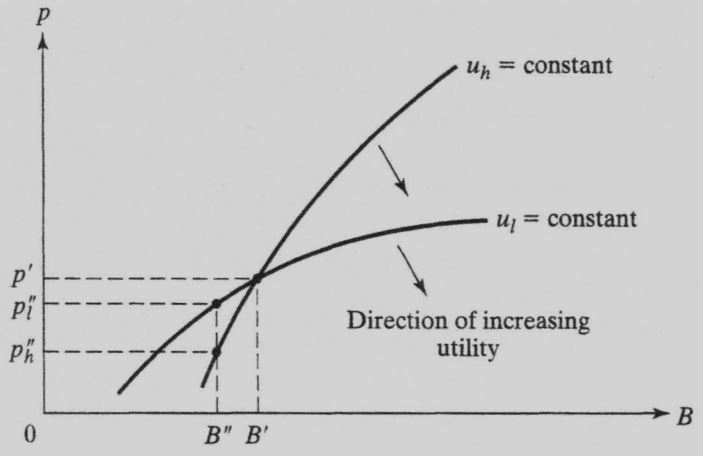
\includegraphics[scale=0.5]{images/advselecutil}
\end{center}

On the side of insurance companies, we can use the previous graph to describe three types of contracts $\psi$. First, all contracts below the line $p = \ubar\pi B$ are not profitable for the insurance company. All contracts above the line $p = \bar\pi B$ are profitable to the insurance company regardless of the type of consumer that buys the policy. Between both lines, the contracts are profitable only if bought by low types. Graphically, we have:\begin{center}
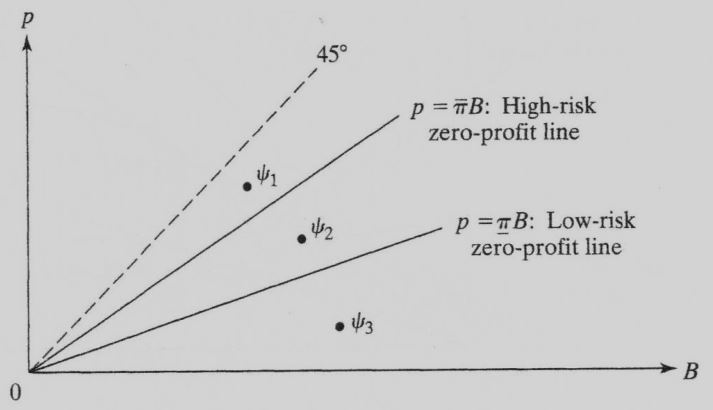
\includegraphics[scale=0.5]{images/advselecprofit}
\end{center}

\subsubsection{Perfect Bayesian Equilibria}

Let $(\psi_l, \psi_h, s(\cdot), \mu(\cdot))$ be a perfect Bayesian equilibrium, where $\mu(B,p)$ is the equilibrium belief of the insurance company that the consumer offering the contract $\psi = (B,p)$ is of the low-risk type. $s(B,p)$ is the action of the insurance company when a consumer offers $\psi = (B,p)$. Denote $u_l^*$ and $u_h^*$ the equilibrium utilities of low-risk and high-risk types respectively. Then it must be that:\begin{itemize}
\item $u_l^* \geq \tilde u_l$ where $\tilde u_l$ is the utility that the low-risk type would get if he was maximizing his utility as a high-risk type.
\item $u_h^* \geq u_h^C$ where $u_h^C \equiv u_h(L, \bar\pi L)$. 
\end{itemize}

\subsubsection{Pooling PBE}



\subsubsection{Separating PBE}

The policies $\psi_l = (B_l, p_l)$ and $\psi_h = (B_h, p_h)$ proposed by the low-risk and high-risk consumers respectively are accepted by the insurance company as a separating equilibrium if and only if:\begin{itemize}
\item $\psi_l\neq\psi_h = (L,\bar\pi L)$: the two contracts are different and the high-risk asks for his full information contract.
\item $p_l\geq \ubar\pi B_l$: the price of the low-risk contract must be such that they have no incentive to refuse.
\item $u_l(\psi_l)\geq \tilde u_l\equiv \max_{(B,p)} u_l(B,p)\text{ s.t. } p = \bar\pi B$: utility from the low-risk contract must be higher than what he would get if he passed as a high-risk.
\item $u_h^C \equiv u_h(\psi_h)\geq u_h(\psi_l)$: utility from the high-risk contract must be higher than what he would get if he passed as a low-risk.
\end{itemize} Graphically, this means that the high-risk asks for a contract that corresponds to his full-information equilibrium while the low-risk type will ask for any contract in the shaded area (graph below), as long as the beliefs of the insurance company are that any other contract proposed would be from a high-risk type.\begin{center}
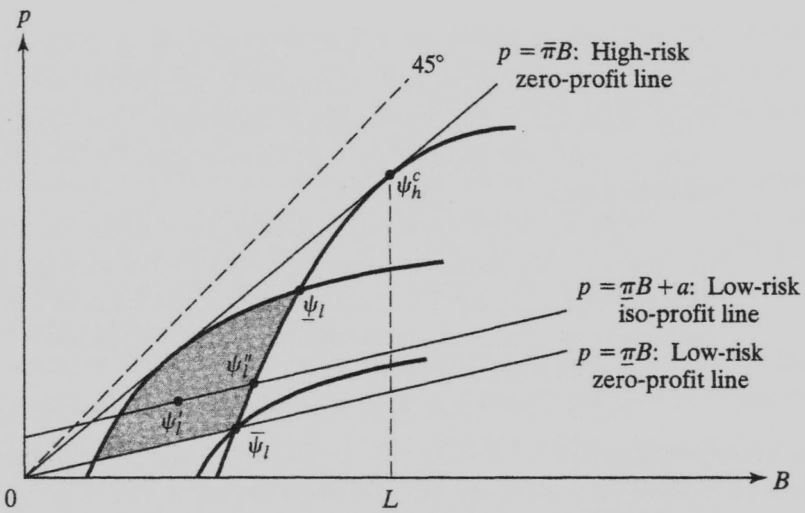
\includegraphics[scale=0.5]{images/advselecsep}
\end{center}

Proof ...

There are some issues of credibility in this previous definition of an equilibrium. Recall that all contract offers from low-risk types must be in the shaded area. However not all contracts are equal in this zone as for all contracts $\psi_l'$ that are not on the $u_h^C$, there exists a contract $\psi_l''$ on $u_h^C$ such that, at the same profit for the insurance company, $\psi_l''$ yields a higher profit for the low-risk consumer, while still being unattractive for the high-risk: we have found a PBE that Pareto dominates another PBE.

Thus, we are left with an infinite number of Pareto-undominated separating equilibria defined by the curve between $\bar\psi_l$ and $\ubar\psi_l$. 

\subsubsection{Intuitive criterion}

We have seen that there exist many equilibria, both pooling or separating, but some of them make no intuitive sense. For example, in separating equilibria, any other contract offer in the shaded area should be believable as they are all below the equilibrium payoff of high-risk consumers. In order to eliminate these non-reasonable equilibria, we need to add a requirement to the PBE so that it weeds out all non-reasonable PBE.

\begin{definition}[Intuitive Criterion]
A PBE $(\psi_l, \psi_h, s(\cdot), \mu(\cdot))$ yielding the utilities $u_l^*, u_h^*$ for low-risk and high-risk types respectively is said to satisfy the IC if for every policy $\psi \neq \psi_l$ and $\psi_h$ with $u_i(\psi) > u_i^*$ and $u_j(\psi) < u_j^*$, then $\mu(\cdot)$ places probability $1$ on risk type being $i$.
\end{definition} This IC means that for all other contracts $\psi$ than the equilibrium ones such that type $i$ prefers $\psi$ and the other does type does not, then the insurance company should logically believe that $i$ is the type proposing $\psi$.

By the intuitive criterion, only one separating PBE can subsist: $(\bar\psi_l,\psi_h^c)$.

\subsection{Screening solution}



\section{Moral Hazard}


\end{document}
